% !TEX program = xelatex
\documentclass[bachelor,openright,notchinese]{sustcthesis}
% 默认twoside 双面打印
% 将master修改为bachelor, doctor or master
% 要使用adobe字体,添加adobefonts选项
% 使用euler数学字体,如不愿使用,去掉euler
% 使用外文写作,请添加notchinese

% 设置图形文件的搜索路径
\graphicspath{{figures/}}
\setboolean{@twoside}{false}

% 用到的宏包
\usepackage{algorithm2e}
\usepackage{scrextend}
% 阻止hyperref宏包影响tableofcontent内容
\makeatletter
\let\Hy@linktoc\Hy@linktoc@none
\makeatother

%%%%%%%%%%%%%%%%%%%%%%%%%%%%%%
%% 封面部分
%%%%%%%%%%%%%%%%%%%%%%%%%%%%%%
 % 中文封面内容
  \title{毕业论文}%一般情况下扉页和封皮、书脊共用一个标题文本,可以不用定义\spinetitle(仅硕博有用), \covertitle(本硕博均有用)和\encovertitle(仅本科有用)。特殊情况见下。
  %特殊情况1:本例中\title命令里含有换行控制字符,这会导致制作书脊的时候出现错误,例如如果你注释掉\spinetitle{...}这一行就会报错。这时需要定义一个不含换行等命令的\spinetitle,这并不表示\spinetitle里不能有任何命令——只能使用有限的命令。
  %特殊情况2:本例中标题过长,所以需要缩小书脊标题的字号。
  %特殊情况3:本例中中英文混排,由于tex竖排的原理限制,中英文基线不重合,所以需要人工调整英文的基线。具体调整量根据不同字体有所不同。
%   \covertitle{六次循环域}
%   \covertitle{中文题目第一行\\中文题目第二行}
  %不要在此调整封皮字体大小! Do not set Cover Page font size here!
  %特殊情况4:本例中\title中含有多个换行,导致标题超过了两行。根据制本厂规定,封皮标题不能超过两行。因此需要定义封皮使用的标题\covertitle. 如果你注释掉这一行,就会发现封皮不符合规定。
  %\encovertitle{On Cyclic Sextic Fields}
  %不要在此调整封皮字体大小! Do not set Cover Page font size here!
  %特殊情况5:仅本科生有用。本科封皮中有英文标题,不超过三行。与上类似。
  \author{田 \ 闰心 }
  \depart{计算机科学与工程}%系别,硕博请用系代号,本科请用全称如
  \major{计算机专业}%专业,硕博请用全称,本科不需要
  \advisor{张进 \ 教授}
  % \coadvisor{XXX\ 教授,\ XXX\ 教授}%第二导师,没有请注释掉
  \studentid{11610734}%For bachelor only
  \submitdate{二〇二〇年三月}

  % 英文封面内容
% \encovertitle{English Title Line 1\\English Title Line 2\\English Title Line 3}
  \entitle{A Bidding Based\\Wireless Resource Allocation\\Using Blockchain Smart Contract} % Bachelor
  \enauthor{Tian Runxin}
  \studentid{11610734}
  \endepart{Computer Science and Engineering}
  \enmajor{Computer Science}
  \enadvisor{Prof. Zhang Jin}
  % \encoadvisor{}
  % \encoadvisorsec{}
  \ensubmitdate{March, 2020}
  
\begin{document}

% 封面
\maketitle

%特别注意,以下述顺序为准,在对应部分添加文档部件,切勿颠倒顺序:
%本科论文的文档部件顺序是:
%    frontmatter:致谢、目录、中文摘要、英文摘要、
%    mainmatter: 正文章节
%    backmatter: 参考文献或资料注释、附录
%%%%%%%%%%%%%%%%%%%%%%%%%%%%%%
%% 前言部分
%%%%%%%%%%%%%%%%%%%%%%%%%%%%%%
\frontmatter
\makeatletter

\ifustc@bachelor
	%%%%%%%%%%%%%%%%%
	%本科论文修改这里
	%%%%%%%%%%%%%%%%%
	% 致谢
	\chapter*{诚信承诺书}
\label{chap:honest}

\begin{enumerate}
\item 本人郑重承诺所呈交的毕业设计(论文),是在导师的指导下,独立进行研究工作所取得的成果,所有数据、图片资料均真实可靠。
\item 除文中已经注明引用的内容外,本论文不包含任何其他人或集体已经发表或撰写过的作品或成果。对本论文的研究作出重要贡献的个人和集体,均已在文中以明确的方式标明。
\item 本人承诺在毕业论文(设计)选题和研究内容过程中没有抄袭他人研究成果和伪造相关数据等行为。
\item 在毕业论文(设计)中对侵犯任何方面知识产权的行为,由本人承担相应的法律责任。
\end{enumerate}

\vskip 3\baselineskip


\begin{flushright}

作者签名: \underline{\hspace{4cm}}
\vskip \baselineskip
\underline{\hspace{1.4cm}}年\underline{\hspace{0.7cm}}月\underline{\hspace{0.7cm}}日

\end{flushright}



    %\chapter{Preface}
\label{chap:chap-preface}
\vskip 28pt

This thesis is made as a completion of the bachelor education in SUSTech.
The thesis is the product of the bachelor period, which is the last part
of the Computer Science study at SUSTech, Computer Science and Engineering
Department.

Several persons have contributed with support to this bachelor thesis. 
Firstly, I would like to thank my supervisor Zhang Jin and co-supervisor
Richar Ma at NUS for their time, valuable suggestions and support throughout 
the period.

Furthermore, I would like to thank Shi Lianjie at NUS for his big help 
through the entire process.

Finally, I would like to thank my family, friends, and girlfriend for being
helpful and supportive during my time studying Computer Science at SUSTech.

\begin{flushright}

Tian Runxin

March, 2020 at SUSTech

\end{flushright}
	
	
	%目录部分
	%目录
	\tableofcontents
	%默认表格、插图、算法索引名称分别为“表格索引”、“插图索引”和“算法索引”
	%如果需要自行修改lot,lof,loa的名称,请定义
	%\ustclotname{...}
    %\ustclofname{...}
	%\ustcloaname{...}

	% 表格索引
	%\ustclot
	% 插图索引
	%\ustclof
	%算法索引 
	%如果需要使用算法环境并列出算法索引,请加入补充宏包。
	%\ustcloa
	
	% 摘要
	\begin{cnabstract}
基于竞价的无线资源分配可以根据用户的需求和网络系统带宽的使用情况来计算网络带宽的价格,并通过集中竞价通过用户的价格参数进行带宽资源的协商和分配。而本文的资源分配思想是基于Kelly机制,它允许用户根据自己的需求获取带宽。通常,竞价系统运行在集中式服务器上,该系统易于设计,但可能具有许多隐藏的安全风险,包括透明性,数据互操作性风险,网络隐私和安全漏洞。

区块链是一种可以轻松解决这些风险的技术,可用于确保交易不可修改且不可否认。另外,由于我们在路由器的边缘部署了竞价和带宽控制系统,因此,在将系统应用于由许多路由器组成的企业网络时,区块链也显示出极大的弹性。在本文中,我们建立了具有新的权威证明机制的私有区块链网络,该机制可以在路由器等边缘设备中以低能耗达成共识。平均而言,与传统的区块链系统相比,采用新型共识算法的区块链系统的响应时间缩短了xx%,电池消耗的电量减少了xx%。

总之,这片文章提出了一个基于区块链智能合约实现的竞价无线资源分配系统。为了使得模型更贴近真实场景,本文以公共区域的Wi-Fi认证与带宽分配系统作为特定的无线资源进行分配。但是,由于不同类型的无线资源间具有相似的用户场景和很高的结构相似度,本文提出并实现的系统可经过较少的改变使其适用于别的无线资源如:4G和5G等等。

\keywords{资源分配, 区块链,智能合约,共识算法}
\end{cnabstract}

\begin{enabstract}

The bidding based wireless resource allocation calculates the price of network bandwidth according to the user's demand and the usage of network system bandwidth and carries out the negotiation and allocation of bandwidth resources through the user's price parameters through centralized bidding. And the resource allocation idea of this paper is based on the Kelly mechanism\cite{yang_price_2013}, which allows users to acquire bandwidth according to their demand. Normally, a bidding system is running on a centralized server, which is easy to design but may have many hidden security risks including transparency, risks of data interoperability, network privacy and security vulnerabilities.

Blockchain, a technology that can easily solve these risks , can be used to ensure transactions are unmodifiable and undeniable. Also, as we deploy the bidding and bandwidth control system on the edge - the router, blockchain also shows great elasticity while applying the system on an enterprise network consisting of many routers. In this paper, we establish a private blockchain network with a new Proof of Authority mechanism, which can reach consensus with low energy consumption in edge devices like a router. On average, the blockchain system with the new consensus algorithm shows xx\% less response time and xx\% less battery power consumed when compared with traditional blockchain systems.

In short, this paper proposes a bidding based wireless resource allocation system using blockchain smart contracts. In order to make the model closer to the real scene, this paper uses the Wi-Fi authentication and bandwidth allocation system in the public area as a specific wireless resource for allocation. However, due to similar user scenarios and high structural similarity between different types of wireless resources, the system proposed and implemented in this paper can be adapted to other wireless resources such as 4G and 5G with few changes.

Keywords: resource allocation, blockchain, smart contract, consensus algorithm


\enkeywords{resource allocation, blockchain, smart contract, consensus algorithm}
\end{enabstract}
%此文件中含有中英文摘要
%   \begin{denotation}
\item[$\mathbb{Q}$] rational number field
\end{denotation}

    
\else
	%%%%%%%%%%%%%%%%%
	%硕博论文修改这里
	%%%%%%%%%%%%%%%%%
	% 摘要
	\begin{cnabstract}
基于竞价的无线资源分配可以根据用户的需求和网络系统带宽的使用情况来计算网络带宽的价格,并通过集中竞价通过用户的价格参数进行带宽资源的协商和分配。而本文的资源分配思想是基于Kelly机制,它允许用户根据自己的需求获取带宽。通常,竞价系统运行在集中式服务器上,该系统易于设计,但可能具有许多隐藏的安全风险,包括透明性,数据互操作性风险,网络隐私和安全漏洞。

区块链是一种可以轻松解决这些风险的技术,可用于确保交易不可修改且不可否认。另外,由于我们在路由器的边缘部署了竞价和带宽控制系统,因此,在将系统应用于由许多路由器组成的企业网络时,区块链也显示出极大的弹性。在本文中,我们建立了具有新的权威证明机制的私有区块链网络,该机制可以在路由器等边缘设备中以低能耗达成共识。平均而言,与传统的区块链系统相比,采用新型共识算法的区块链系统的响应时间缩短了xx%,电池消耗的电量减少了xx%。

总之,这片文章提出了一个基于区块链智能合约实现的竞价无线资源分配系统。为了使得模型更贴近真实场景,本文以公共区域的Wi-Fi认证与带宽分配系统作为特定的无线资源进行分配。但是,由于不同类型的无线资源间具有相似的用户场景和很高的结构相似度,本文提出并实现的系统可经过较少的改变使其适用于别的无线资源如:4G和5G等等。

\keywords{资源分配, 区块链,智能合约,共识算法}
\end{cnabstract}

\begin{enabstract}

The bidding based wireless resource allocation calculates the price of network bandwidth according to the user's demand and the usage of network system bandwidth and carries out the negotiation and allocation of bandwidth resources through the user's price parameters through centralized bidding. And the resource allocation idea of this paper is based on the Kelly mechanism\cite{yang_price_2013}, which allows users to acquire bandwidth according to their demand. Normally, a bidding system is running on a centralized server, which is easy to design but may have many hidden security risks including transparency, risks of data interoperability, network privacy and security vulnerabilities.

Blockchain, a technology that can easily solve these risks , can be used to ensure transactions are unmodifiable and undeniable. Also, as we deploy the bidding and bandwidth control system on the edge - the router, blockchain also shows great elasticity while applying the system on an enterprise network consisting of many routers. In this paper, we establish a private blockchain network with a new Proof of Authority mechanism, which can reach consensus with low energy consumption in edge devices like a router. On average, the blockchain system with the new consensus algorithm shows xx\% less response time and xx\% less battery power consumed when compared with traditional blockchain systems.

In short, this paper proposes a bidding based wireless resource allocation system using blockchain smart contracts. In order to make the model closer to the real scene, this paper uses the Wi-Fi authentication and bandwidth allocation system in the public area as a specific wireless resource for allocation. However, due to similar user scenarios and high structural similarity between different types of wireless resources, the system proposed and implemented in this paper can be adapted to other wireless resources such as 4G and 5G with few changes.

Keywords: resource allocation, blockchain, smart contract, consensus algorithm


\enkeywords{resource allocation, blockchain, smart contract, consensus algorithm}
\end{enabstract}
%此文件中含有中英文摘要
	% 目录
	\tableofcontents
	%默认表格、插图、算法索引名称分别为“表格索引”、“插图索引”和“算法索引”
	%如果需要自行修改lot,lof,loa的名称,请定义
	%\ustclotname{...}
	%\ustclofname{...}
	%\ustcloaname{...}

	% 表格索引
	\ustclot
	% 插图索引
	\ustclof
	%算法索引 
	%如果需要使用算法环境并列出算法索引,请加入补充宏包。
	%\ustcloa
	
	%符号说明,需要加入补充包
	\begin{denotation}
\item[$\mathbb{Q}$] rational number field
\end{denotation}
%不是必需的,如果不想列出请注释掉
\fi
\makeatother

%%%%%%%%%%%%%%%%%%%%%%%%%%%%%%
%% 正文部分
%%%%%%%%%%%%%%%%%%%%%%%%%%%%%%
\mainmatter
  \chapter{Introduction}
\label{chp:introduction}

\section{Background}

Over the past few decades, wireless communications and networking have experienced an unprecedented growth. However, along with the growth of wireless network technology, the number of active users and the Big Data on the Internet also experienced a near-exponential growth. Which bring many challenges to wireless resource allocation, such as limited wireless resources, differ multi-user need and trad-offs among multi-user service objectives \cite{wang_blockchain-based_2019}. 

To overcame these challenges, dynamic resource allocation is used to improve the overall system performance and ensure individual Quality of Service (QoS), which concerns about bandwidth capacity allocation. In practice, one of the biggest challenges of these problems is the system naturally does not know the characteristics of users and their applications. Moreover, the users are often autonomous and selfish, and they may misreport their real needs to maximize their own utilities. 

To mitigate the above problems, resource pricing mechanisms have been introduced to manage resource allocation. In this work, we use generalized Kelly mechanism with price differentiation mechanism\cite{yang_price_2013} by R.M, which allows autonomous resource owners to apply different price differentiation schemes so as to achieve individual objectives, e.g., making trade-offs between user fairness and system efficiency. The generalized mechanism extends the flexibility of the Kelly mechanism and it is also adaptive and robust, since the mechanism depends on a congestion pricing principle and the allocations are implemented as Nash equilibrium solutions.

In order to avoid the security risks brought by running mentioned resource allocation mechanism on a central server, blockchain technology, a promising technology to address trust and security concerns, is apply to deploy the generalized Kelly mechanism as a smart contract. Which can be used to ensure the related transactions are unmodifiable and undeniable, and make the overall service open and transparent.

\textbf{In this work, a bidding based wireless resource allocation system is proposed, which consist of a "serverless" web application, a a smart contract and private blockchain node.} For quick verification purpose, the bandwidth control is implemented by running a python script to maintain a IP table of active users. To make the system more closer to industrial use, I will try to use a captive portal to do the wireless network control and monitoring.

\section{Related Works}

\textbf{Resource allocation mechanism are wide need over computing resources}, e.g., computing services, network resources and content streaming services, have been studied extensively during the last decade. And due to the characteristics of blockchain, scholars have conducted related research on the combination of blockchain technology with cloud computing, fog computing and edge computing, including research with the Internet of Things, access control technology and other related fields. This thesis focuses on resource allocation in a edge computing environment. Both the blockchain node and captive portal run on a router or a Respberry Pi.

WANG H, et al.\cite{wang_blockchain-based_2019} proposed a resource contribution model between the fog node and cloud or users, which practices the reward and punishment mechanism of the blockchain to boost the fog nodes to contribute resources actively. With the behavior of the fog node in contributing resources are stored in the blockchain, a transparent, open and tamper-free service evaluation index forms. In their model, the designed reward and punishment mechanism is very similar with the mining activity of miners.

LIU M, et al.\cite{liu_distributed_2019} proposed a blockchain-based video streaming system, aiming to build decentralized peer-to-peer networks with flexible monetization mechanisms for video streaming services. In this thesis, the author designed a novel blockchain-based framework with adaptive block size for video streaming with mobile edge computing.

% ABDELLATIF K, ABDELMOUTTALIB C.  TO BE DECIDED.

\section{Motivation and Contributions}

\textbf{The main motivation of this work is to show how blockchain system could help with resouce allocation,} how  smart contract could provide bidding or pricing based system avoid security risks and achieve indeed transparency and unmodifiable properties. And theoretically, the bandwidth capacity of wireless network, an example wireless resource, can be easily replace with any other wireless resource with few modification. 

\textbf{The contributions of this work are} 1. proposed and designed a bidding/pricing based resource allocation system on smart contract, 2. implemented a practical system focus on wireless bandwidth capacity allocation, 3. built a private PoA blockchain network and plan to evaluate the performance difference with PoW network.

\section{Thesis Structure}

This thesis is organised as follows:
In Chapter. 2, the model design of the overall system is shown.
Then, the generalized Kelly mechanism is introduced in detail in Chapter. 3. 
In Chapter. 4, the blockchain related terms such as "Smart Contracts", "Consensus Algorithm" and "DApp" are introduced in detail. 
Subsequently, my implementation of the system and challenging problems I faced during implementation are presented in Chapter. 5. 
At last, some performance evaluation and comparison are made in Chapter. 6.

	
  %自行添加
  \chapter{Preliminaries}
\label{chp:chap-two}

\section{Resource Allocation Mechanism}

In this session, the resource allocation mechanism used by our system will be introduced, and the reason we select it will be discussed as follow\cite{yang_price_2013}.

\subsection{The Kelly Mechanism}

In this section, we give some background about the Kelly mechanism and further generalize it by using an embedded price differentiation. In the next section, we will explore the properties of the generalized mechanisms.

We consider a set $N=|\mathscr{N}|>1$ of rational users bidding for a share of divisible resource of capacity $C$. We assume that more than one user compete for the resource, i.e., $N=|\mathscr{N}|>1$. Each user i has a valuation function $v_{i}(\cdot)$, where $v_{i}\left(d_{i}\right)$ defines the monetary utility to user i when she is given $d_{i}$ amount of the resource.

A common objective in resource allocation is to maximize the social welfare. Under our context, it is to maximize the sum of the valuations of all the users as the following optimization problem:

\begin{itemize}
\item max           $\sum_{i \in \mathcal{N}} v_{i}\left(d_{i}\right)$
\item subject to    $\sum_{i \in \mathcal{N}} d_{i} \leq C \quad$ and $\quad d_{i} \geq 0 \forall i \in \mathcal{N}$
\end{itemize}

We define the above convex and compact constraint set as
$$
\mathscr{D}=\left\{\mathbf{d} | \sum_{i \in \mathcal{N}} d_{i} \leq c, \text { and } d_{i} \geq 0, \forall i \in \mathcal{N}\right\}
$$
In the Kelly mechanism [1] , each user $i$ submits a bid $w_{i} \geq 0$, which equals the payment for obtaining a share $d_{i}$ of the resource. We denote $u_{i}$ as the utility of each user $i$, defined in a quasi-linear [12] environment as $u_{i}\left(d_{i}\right)=v_{i}\left(d_{i}\right)-w_{i}$
which is the valuation of the allocated resource $v_{i}\left(d_{i}\right)$ less the payment $w_{i}$. The Kelly mechanism allocates the full capacity
C among all users and the resource share $d_{i}$ of each user $i$ is proportional to her bid $w_{i} .$ Mathematically, given a nonzero bid vector $\mathbf{w}=\left(w_{1}, w_{2}, \ldots, w_{N}\right),$ the resource allocation vector $\mathbf{d}=\left(d_{1}, d_{2}, \ldots, d_{N}\right)$ is defined by
$$
d_{i}=D_{i}(\mathbf{w})=\frac{w_{i}}{\sum_{j=1}^{N} w_{j}} c, \quad \forall i \in \mathcal{N}
$$
where $D_{i}(\cdot)$ denotes the proportional allocation function for user $i$ under the Kelly mechanism.

As a result of the Kelly mechanism, each user is charged the same unit price of the resource $\mu$ such that $\mu d_{i}=w_{i}$ for all users. This implicit unit price $\mu$ can be calculated as
$$
\mu=\frac{\sum_{j=1}^{N} w_{j}}{c}
$$

\subsection{The Generalized Kelly Mechanism}

Rather than implementing a nondiscriminatory price $\mu$ under the Kelly mechanism, we consider a price differentiation among users. Our motivation of designing the price differentiation is to achieve different efficiency points for the social welfare defined as the objective function of (1). Under our generalization, we consider a strict positive price vector $\mathbf{p}=$ $\left(p_{1}, p_{2}, \ldots, p_{N}\right)$ as a parameter of the mechanism. Each user $i$ submits a bid $t_{i} \geq 0$ to compete for the resource and the allocation rule is the same proportional rule defined in Eq. (2):
$$
d_{i}=D_{i}(\mathbf{t})=\frac{t_{i}}{\sum_{j=1}^{N} t_{j}} c, \quad \forall i \in \mathcal{N}
$$
The difference of our generalization from the Kelly mechanism is that each user i pays $p_{i} t_{i}$ amount of money for $D_{i}(\mathbf{t})$ amount
of shared resource, and therefore, obtains a utility of $u_{i}(\mathbf{t}, \mathbf{p})=v_{i}\left(d_{i}\right)-p_{i} t_{i}=v_{i}\left(D_{i}(t)\right)-p_{t} t_{i}$
This generalized mechanism can be imagined as a process where users buy divisible tickets to compete for the resource. We denote $t_{i}$ as the number of tickets bought by user $i$ and $p_{i}$ as the monetary price of each ticket for user i. Like the Kelly mechanism, it fully allocates the capacity $C$ among all users and the resource share $d_{i}=D_{i}(\mathbf{t})$ to each user $i$ is proportional to the number of tickets bought: $t_{i .}$ Although we do not differentiate tickets in resource allocation, the unit ticket price to users could be different. In particular, the Kelly mechanism is a special case of the generalization where $\mathbf{p}=1$

Compared to the Kelly mechanism, the generalized mechanism achieves a similar virtual unit price $v$ in terms of tickets (measured as tickets per unit of resource) defined as $v=\frac{\sum_{j=1}^{N} t_{j}}{c}$
Consequently, the effective/real unit price for resource among users will be proportional to the price vector $\mathbf{p},$ because each user i's real price becomes $p_{i} v$ (measured as abstract monetary units per unit of resource). Notice that although a pre-determined price is assigned to each user, the generalized mechanism inherits the simplicity/scalability of the Kelly mechanism in two ways: ( 1) the strategy space of the mechanism is still simply one-dimensional; and ( 2 ) only a single virtual price feedback, i.e., $v$, is required to be sent to all users.

\section{Blockchain Concepts}

In this session, the basic definitions of Blockchain related terms are discussed in details, such as DApp, Smart Contract and Consensus Algorithm.

\subsection{What is DApp}

First of all, since our proposed system is a DApp\cite{johnston_general_nodate}, the DApp is introduced as follow. 

\subsubsection{Definition}

For an application to be considered a DApp, it must meet the following criteria:

\begin{enumerate}
\item The application must be completely open-source, it must operate autonomously, with no entity controlling the majority of its tokens, and its data and records of operation must be crypto graphically stored in a public, decentralized block chain.
\item The application must generate tokens according to a standard algorithm or set of criteria and possibly distribute some or all of its tokens at the beginning of its operation. These tokens must be necessary for the use of the application and any contribution from users should be rewarded by payment in the application’s tokens.
\item The application may adapt its protocol in response to proposed improvements and market feedback but all changes must be decided by majority consensus of its users.
\end{enumerate}

\subsubsection{The Bitcoin}

The Bitcoin, the most famous DApp, is described as "A Peer-to-Peer Electronic Cash System\cite{nakamoto_bitcoin_nodate}" by Satoshi Nakamoto. Bitcoin has been shown to effectively solve the problems that arise from a trustless and scalable electronic cash system by using a peer-to-peer, distributed ledger, the Bitcoin block chain. In addition to being a peer-to-peer electronic cash system however, Bitcoin is also an application that users can interact with through computer software). But most importantly for the purposes of this paper, based on the criteria outlined above, Bitcoin is a decentralized application. Here is why:

\begin{enumerate}
\item All Bitcoin software applications are open-source, no entity (government,company, or organization) controls Bitcoin and all records related to the use of Bitcoin are open and public.
\item Bitcoin generates its tokens, the bitcoins, with a predetermined algorithm that cannot be changed, and those tokens are necessary for Bitcoin to function. Bitcoin miners are rewarded with bitcoins for their contributions in securing the Bitcoin network.
\item All changes to Bitcoin must be approved by a majority consensus of its users through the proof-of-work mechanism.
\end{enumerate}

\subsection{Smart Contract}

A smart contract is a computer program that both expresses the contents of a contractual agreement and operates the implementation of that content, on the basis of triggers provided by the users or extracted from the environment. Smart contracts are currently promoted as means to leverage efficiency, security and impartiality in the execution of an agreement, thereby reducing the costs in implementing contracts and increasing trust between parties.

Practically, smart contracts are in charge of reading and writing data to the Blockchain, as well as executing business logic. Smart contacts are written in a programming language called Solidity, which looks a lot like Javascript.

In the case of our bidding DApp, it is an agreement that my bidding payment will count, that the Kelly mechanism controls the bidding result, and that every user would get corresponding resource - the bandwidth precisely.

\subsection{Consensus Algorithm}

We know that Blockchain is a distributed decentralized network that provides immutability, privacy, security, and transparency. There is no central authority present to validate and verify the transactions, yet every transaction in the Blockchain is considered to be completely secured and verified. This is possible only because of the presence of the consensus protocol which is a core part of any Blockchain network. 

https://www.geeksforgeeks.org/consensus-algorithms-in-blockchain/

A consensus algorithm is a procedure through which all the peers of the Blockchain network reach a common agreement about the present state of the distributed ledger. In this way, consensus algorithms achieve reliability in the Blockchain network and establish trust between unknown peers in a distributed computing environment. Essentially, the consensus protocol makes sure that every new block that is added to the Blockchain is the one and only version of the truth that is agreed upon by all the nodes in the Blockchain.

The Blockchain consensus protocol consists of some specific objectives such as coming to an agreement, collaboration, co-operation, equal rights to every node, and mandatory participation of each node in the consensus process. Thus, a consensus algorithm aims at finding a common agreement that is a win for the entire network.

\subsubsection{Proof of Work}

The Proof-of-Work (PoW) is used to select a miner for the next block generation. Bitcoin uses this PoW consensus algorithm. The central idea behind this algorithm is to solve a complex mathematical puzzle and easily give out a solution. This mathematical puzzle requires a lot of computational power and thus, the node who solves the puzzle as soon as possible gets to mine the next block. 

\subsubsection{Proof of Authority}

https://www.coinhouse.com/learn/blockchain/what-is-proof-of-authority/

The Proof-of-Authority (PoA) is a consensus method that gives a small and designated number of blockchain actors the power to validate transactions or interactions with the network and to update its more or less distributed registry. It works as follow: according to the chosen scheme, one or more validating machines are responsible for generating each new block of transactions that will be included in the Blockchain. The new block can be accepted directly without verification, or by unanimous vote of the block generators, or simply by a majority, depending on the configuration chosen for the Blockchain.
  \chapter{System Architecture}
\label{chp:chap-three}

In this chapter, a overview of the system architecture and the design model of the system is introduced in details. Before introducing all the subsystems part by part, a overview architecture of our system is shown in Fig.\ref{fig:system} Our system is a resource allocation system for allocating WiFi bandwidth capacity to users, and use a pricing mechanism to allocate the bandwidth to every user accordingly. And using the blockchain contract, we target to achieve a robust, transparent and user-friendly system.

\begin{figure}[h]
    \centering
    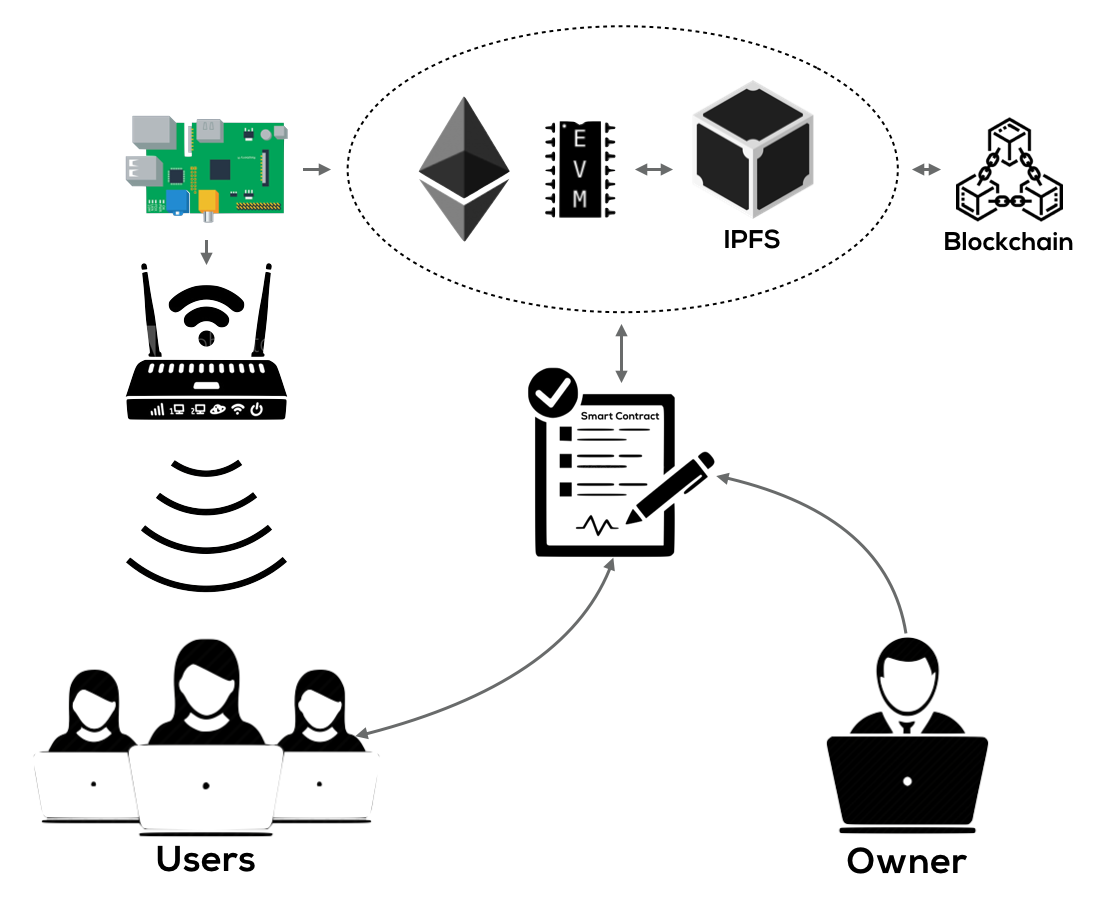
\includegraphics[width=10cm]{My-Thesis/figures/system-architecture.png}    
    \caption{System Architecture}
    \label{fig:system}
\end{figure}

As can be seen from upper Fig.\ref{fig:system}, our system can be mainly divided into two parts -- WiFi Controller and Smart Contract. The two parts currently both are running on the one raspberr pi, whose details would be introduced in Chapter. \ref{chp:chap-five}

\section{WiFi Controller}

\section{Smart Contract}

  \chapter{System Design}
\label{chp:chap-four}

\section{WiFi Controller Design}

\section{Smart Contract Design}

The two major components are the WiFi controller and the smart contract. The smart contract  calculates the bandwidth allocation and collects payments. The WiFi controller allocates the correct bandwidth to each user. Before introducing each part in detail, an analysis is given between system design of traditional app and DApp.

\section{Tradition App and DApp}
Roughly, our proposed system can be considered as a web application with blockchain smart contract, which follows the definition of the DApp\cite{johnston_general_nodate}. DApp, stands for Decentralized Application, which would be introduced in detail in Chapter. \ref{chp:chap-five}. And a typical web application is a group of code such as html, javascript and css. As this group of code running on users' personal devices, a browser, users can interact with the application to fulfill their demands.

And normally when you interact with a web application, you use a web browser to connect to a central server over a network. All the code of this web application lives on this central server, and all the data lives in a central database. Anytime you transact with your application, must communicate with this central server on the web. This is what happened while using the traditional web applications. And the system structure of this kind of web application is shown in  Fig.\ref{fig:app}

\begin{figure}[h]
    \centering
    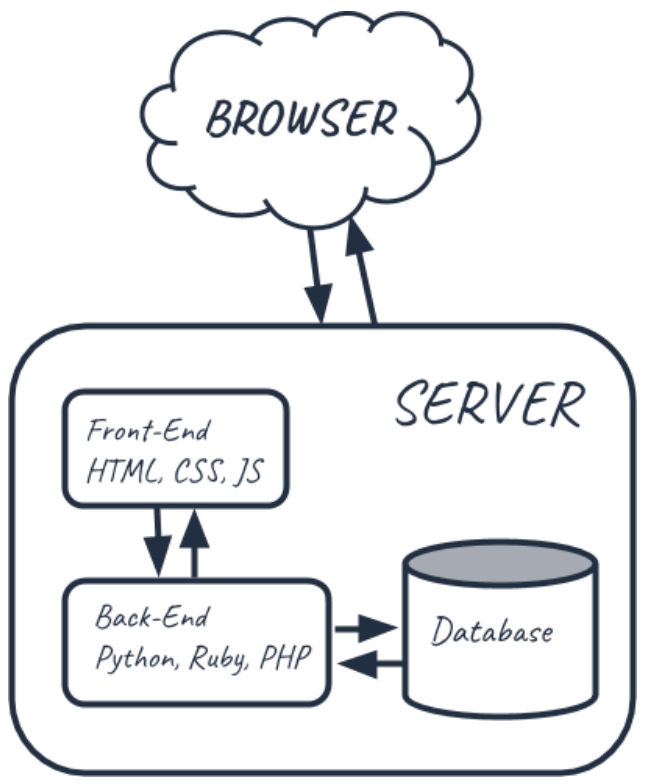
\includegraphics[width=5cm]{My-Thesis/figures/traditional_web_application.png}    
    \caption{Traditional App System Structure}
    \label{fig:app}
\end{figure}
\begin{figure}[h]
    \centering
    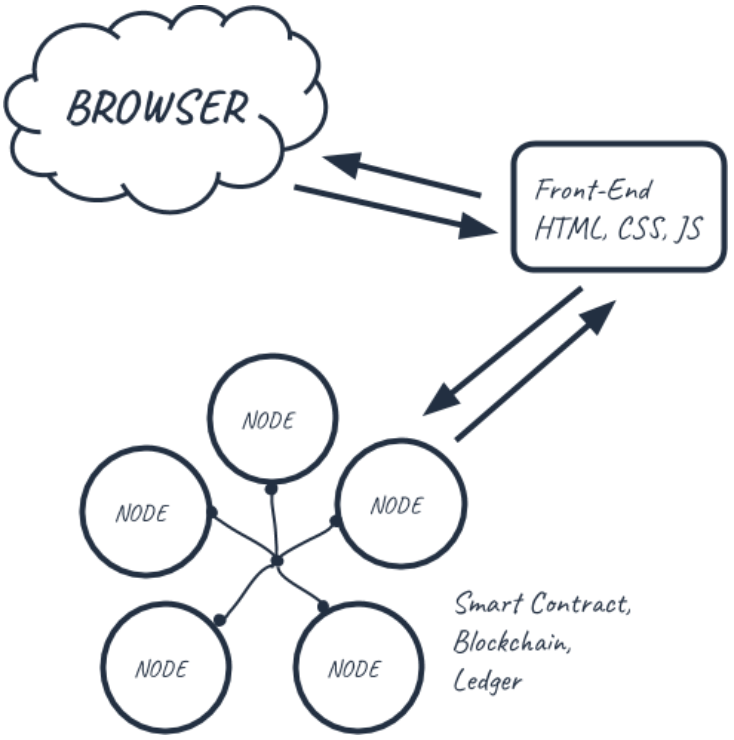
\includegraphics[width=5cm]{My-Thesis/figures/dapp_structure.png}    
    \caption{DApp System Structure}
    \label{fig:dapp}
\end{figure}

And this traditional and widely used kind of web application is very intuitive to develop and holds a great performance while having a powerful central server. However even as concurrent server frameworks are already well developed in decade, a single centralized server always have a limit number of users it can interact with at the same time. And when the central server shut down, the whole system shut down. While, the system structure of a DApp system holds a great elasticity and a robustness while facing the rapidly growing number of user. However, this defect of traditional structure can be solved with a "centralized" distributed servers, which runs the traditional system structure on a distributed group of server instance.

But more importantly, the main reason that the concept DApp was published by scholars is that it can achieve some application scenarios that a traditional app can not support. And in such scenarios, the properties that a traditional web application holds may become the drawbacks. Taking our use case, bidding system, as an example, while implementing the bidding system on a centralized server like Fig.\ref{fig:app}, it will run into two problems as following:
\begin{addmargin}[2em]{0em}

The data on the database could be changed: it could be counted more than once, or removed entirely. \newline The source code on the web server could also be changed at any time.
\end{addmargin}

  \chapter{Implementation and Evaluation}
\label{chp:chap-five}

\section{Implementation Details}

\subsection{WiFi Controller Implementation}



\subsection{Smart Contract Implementation}



\subsection{Development Framework}

Thanks to the rapid development of blockchain technology, both the private blockchain network deployment tools and DApp\cite{johnston_general_nodate} development framework are state of art. My main contributions are model design, private blockchain network deployment, DApp implementation and system evaluation. The state-of-art developing tools and framework I used are:
\begin{enumerate}
\item Go Ethereum (Geth) is one of the three original implementations (along with C++ and Python) of the Ethereum protocol. It is written in Go, fully open source and licensed under the GNU LGPL v3. And Ethereum is a decentralized platform that runs smart contracts, applications that run exactly as programmed without possibility of downtime, censorship, fraud or third party interference. 
\item Remix, a Solidity IDE used to write, compile and debug Solidity code. Solidity, an object-oriented, high-level language for implementing smart contracts. Smart contracts, detailing in Chapter. 3, are programs which govern the behaviour of accounts within the Ethereum state. 
\item Truffe Suite, consisting of Truffle, Ganache and Drizzle. Trufflle is a world class development environment, testing framework and asset pipeline for blockchains using the Ethereum Virtual Machine (EVM). And Ganache is a personal testing blockchain for Ethereum development. And Drizzle, a collection of front-end libraries, take care of synchronizing contract data, transaction data, etc. 
\end{enumerate}

But still, as the technologies are extensively developing, the implementation of the third-party development tools also keep iterating, which may contain some weird bugs more or less. Here are some challenges while developing the system: 
\begin{enumerate}

\item Proof-of-Authority(PoA) blockchain network is still in the early stages of development. Since the most common consensus algorithm is Proof-of-Work, the current PoA network deployment tools only implement PoA like a adapt version of Proof-of-Work. And so the PoA related code may be buggy.
\item The development tools keep changing, during the developing process, the Drizzle development framework suddenly release a new version and the old version was deprecated. So, the messy dependencies also becomes a challenge.
\end{enumerate}

\section{System Evaluation}

Facing these challenges, I actively involved in the development of open source tools themselves, like report issues, review pull requests and make comments on others' work.

\begin{enumerate}
\item Evaluate the transaction time gap between PoW and PoA consensus algorithm.
\item Evaluate the power consumption difference between PoW and PoA consensus algorithm.
\item Verify the correctness of the result according to the generlized Kelly mechanism.
\end{enumerate}

\subsection{Test Cases and Results}

From test cases and results shown in Fig.\ref{fig:test} and Fig.\ref{fig:result}, we could roughly get the average time for a new user join in the system and re-allocation the bandwidth is around 449.8 ms. The response time is short enough for production.

\begin{figure}[h]
    \centering
    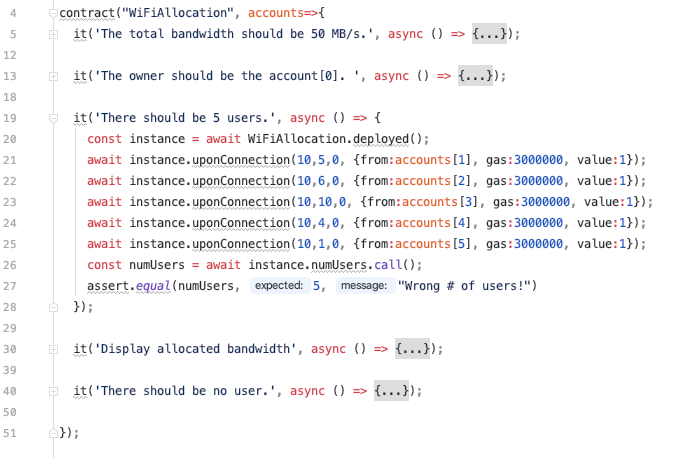
\includegraphics[width=10cm]{My-Thesis/figures/testcases.png}    
    \caption{Test cases}
    \label{fig:test}
\end{figure}

\begin{figure}[h]
    \centering
    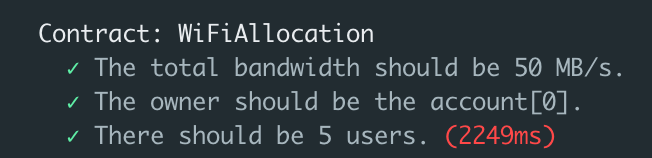
\includegraphics[width=10cm]{My-Thesis/figures/result.png}    
    \caption{Test result}
    \label{fig:result}
\end{figure}

\section{Environment Setup}

The Fig. \ref{fig:environment} shows the experiment environment I used while developing the system. The router is LINKSYS-WRT1900ACS, and the raspberry pi is 4B.

\begin{figure}[h]
    \centering
    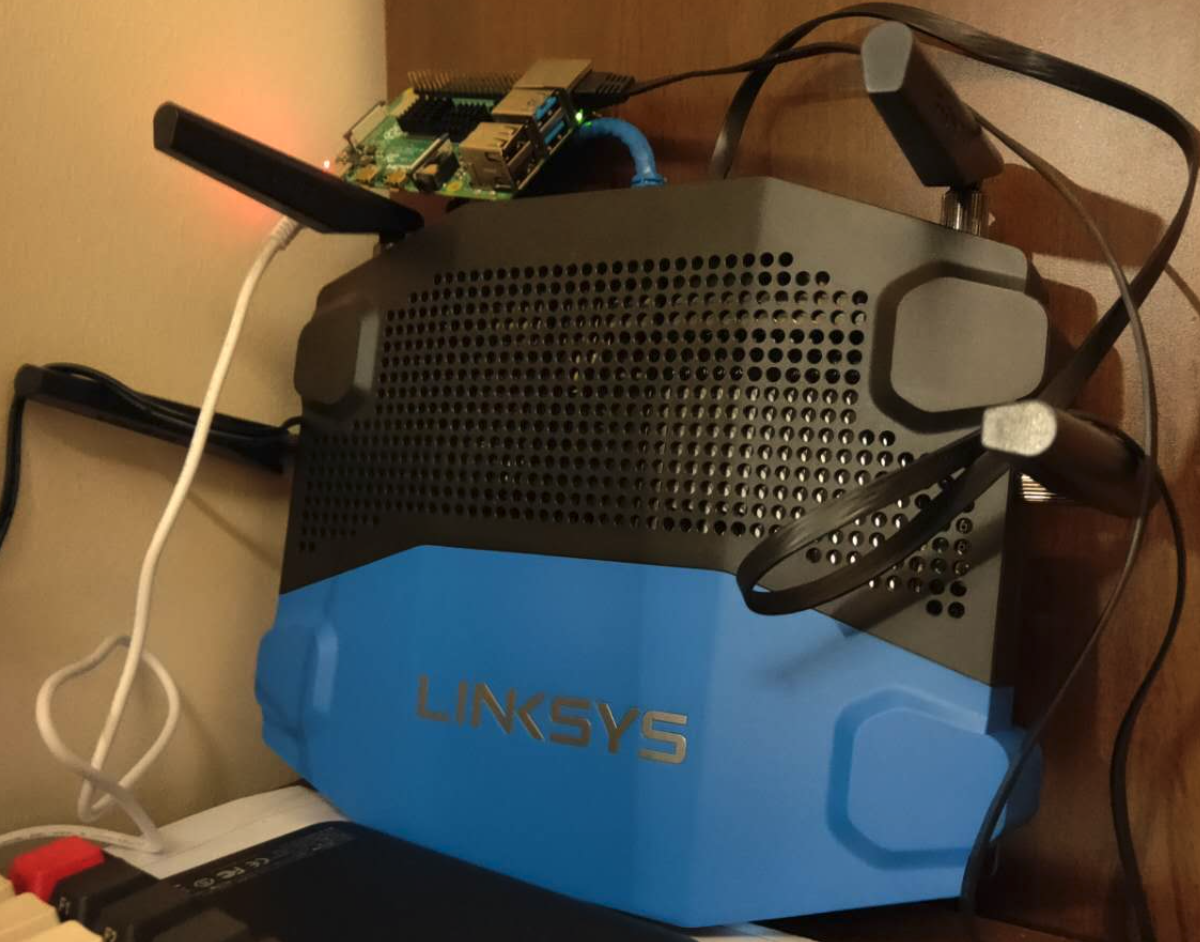
\includegraphics[width=10cm]{My-Thesis/figures/devices.png}    
    \caption{Environment Setup}
    \label{fig:environment}
\end{figure}

  \chapter*{Conclusion}
\label{chp:conclusion}

So far, the implementation of the system is complete. 1. The proposed system runs properly and correctly, 2. It can perfectly follow the Generalized Kelly Mechanism, 3. Using PoA consensus algorithm, the transaction time is short enough for a production system.

\section{Future Plan}

\begin{itemize}
\item Try Captive Portal approach to control the bandwidth
\item Performance Evaluation
    \begin{itemize}
      \item Power consumption
      \item Response time
      \item Correctness
    \end{itemize}
\item More literature review
    \begin{itemize}
        \item More related works to compare and point out the difference and contribution
        \item Divide the related works to two parts
    \end{itemize}{}
\item Finish the thesis
\end{itemize} 


%%%%%%%%%%%%%%%%%%%%%%%%%%%%%%
%% 附件部分
%%%%%%%%%%%%%%%%%%%%%%%%%%%%%%
\backmatter
  %结语
  
  % 参考文献
  % 使用 BibTeX
  % 选择参考文献的排版格式。注意ustcbib这个格式不保证完全符合要求,请自行决定是否使用
  \bibliographystyle{sustcbib}%{GBT7714-2005NLang-UTF8}
  \bibliography{bib/tex}
  \nocite{*} % for every item
  % 不使用 BibTeX
  % \include{chapter/bib}
  % 附录,没有请注释掉
%   \begin{appendix}

%   \chapter{Resource Allocation}
\label{chap:resource}

In this session, the resource allocation mechanism used by our system will be introduced, and the reason we select it will be discussed as follow\cite{yang_price_2013}.

\section{Kelly Mechanism}

In this section, we give some background about the Kelly mechanism and further generalize it by using an embedded price differentiation. In the next section, we will explore the properties of the generalized mechanisms.

We consider a set $N=|\mathscr{N}|>1$ of rational users bidding for a share of divisible resource of capacity $C$. We assume that more than one user compete for the resource, i.e., $N=|\mathscr{N}|>1$. Each user i has a valuation function $v_{i}(\cdot)$, where $v_{i}\left(d_{i}\right)$ defines the monetary utility to user i when she is given $d_{i}$ amount of the resource.

A common objective in resource allocation is to maximize the social welfare. Under our context, it is to maximize the sum of the valuations of all the users as the following optimization problem:

\begin{itemize}
\item max           $\sum_{i \in \mathcal{N}} v_{i}\left(d_{i}\right)$
\item subject to    $\sum_{i \in \mathcal{N}} d_{i} \leq C \quad$ and $\quad d_{i} \geq 0 \forall i \in \mathcal{N}$
\end{itemize}

We define the above convex and compact constraint set as
$$
\mathscr{D}=\left\{\mathbf{d} | \sum_{i \in \mathcal{N}} d_{i} \leq c, \text { and } d_{i} \geq 0, \forall i \in \mathcal{N}\right\}
$$
In the Kelly mechanism [1] , each user $i$ submits a bid $w_{i} \geq 0$, which equals the payment for obtaining a share $d_{i}$ of the resource. We denote $u_{i}$ as the utility of each user $i$, defined in a quasi-linear [12] environment as $u_{i}\left(d_{i}\right)=v_{i}\left(d_{i}\right)-w_{i}$
which is the valuation of the allocated resource $v_{i}\left(d_{i}\right)$ less the payment $w_{i}$. The Kelly mechanism allocates the full capacity
C among all users and the resource share $d_{i}$ of each user $i$ is proportional to her bid $w_{i} .$ Mathematically, given a nonzero bid vector $\mathbf{w}=\left(w_{1}, w_{2}, \ldots, w_{N}\right),$ the resource allocation vector $\mathbf{d}=\left(d_{1}, d_{2}, \ldots, d_{N}\right)$ is defined by
$$
d_{i}=D_{i}(\mathbf{w})=\frac{w_{i}}{\sum_{j=1}^{N} w_{j}} c, \quad \forall i \in \mathcal{N}
$$
where $D_{i}(\cdot)$ denotes the proportional allocation function for user $i$ under the Kelly mechanism.

As a result of the Kelly mechanism, each user is charged the same unit price of the resource $\mu$ such that $\mu d_{i}=w_{i}$ for all users. This implicit unit price $\mu$ can be calculated as
$$
\mu=\frac{\sum_{j=1}^{N} w_{j}}{c}
$$

\section{The Generalized Kelly Mechanism}

Rather than implementing a nondiscriminatory price $\mu$ under the Kelly mechanism, we consider a price differentiation among users. Our motivation of designing the price differentiation is to achieve different efficiency points for the social welfare defined as the objective function of (1). Under our generalization, we consider a strict positive price vector $\mathbf{p}=$ $\left(p_{1}, p_{2}, \ldots, p_{N}\right)$ as a parameter of the mechanism. Each user $i$ submits a bid $t_{i} \geq 0$ to compete for the resource and the allocation rule is the same proportional rule defined in Eq. (2):
$$
d_{i}=D_{i}(\mathbf{t})=\frac{t_{i}}{\sum_{j=1}^{N} t_{j}} c, \quad \forall i \in \mathcal{N}
$$
The difference of our generalization from the Kelly mechanism is that each user i pays $p_{i} t_{i}$ amount of money for $D_{i}(\mathbf{t})$ amount
of shared resource, and therefore, obtains a utility of $u_{i}(\mathbf{t}, \mathbf{p})=v_{i}\left(d_{i}\right)-p_{i} t_{i}=v_{i}\left(D_{i}(t)\right)-p_{t} t_{i}$
This generalized mechanism can be imagined as a process where users buy divisible tickets to compete for the resource. We denote $t_{i}$ as the number of tickets bought by user $i$ and $p_{i}$ as the monetary price of each ticket for user i. Like the Kelly mechanism, it fully allocates the capacity $C$ among all users and the resource share $d_{i}=D_{i}(\mathbf{t})$ to each user $i$ is proportional to the number of tickets bought: $t_{i .}$ Although we do not differentiate tickets in resource allocation, the unit ticket price to users could be different. In particular, the Kelly mechanism is a special case of the generalization where $\mathbf{p}=1$

Compared to the Kelly mechanism, the generalized mechanism achieves a similar virtual unit price $v$ in terms of tickets (measured as tickets per unit of resource) defined as $v=\frac{\sum_{j=1}^{N} t_{j}}{c}$
Consequently, the effective/real unit price for resource among users will be proportional to the price vector $\mathbf{p},$ because each user i's real price becomes $p_{i} v$ (measured as abstract monetary units per unit of resource). Notice that although a pre-determined price is assigned to each user, the generalized mechanism inherits the simplicity/scalability of the Kelly mechanism in two ways: ( 1) the strategy space of the mechanism is still simply one-dimensional; and ( 2 ) only a single virtual price feedback, i.e., $v$, is required to be sent to all users.
%   \chapter{Blockchain}
\label{chap:blockchain}

In this session, the basic definitions of Blockchain related terms are discussed in details, such as DApp, Smart Contract and Consensus Algorithm.

\section{What is DApp}

First of all, since our proposed system is a DApp\cite{johnston_general_nodate}, the DApp is introduced as follow. 

\subsection{Definition}

For an application to be considered a DApp, it must meet the following criteria:

\begin{enumerate}
\item The application must be completely open-source, it must operate autonomously, with no entity controlling the majority of its tokens, and its data and records of operation must be crypto graphically stored in a public, decentralized block chain.
\item The application must generate tokens according to a standard algorithm or set of criteria and possibly distribute some or all of its tokens at the beginning of its operation. These tokens must be necessary for the use of the application and any contribution from users should be rewarded by payment in the application’s tokens.
\item The application may adapt its protocol in response to proposed improvements and market feedback but all changes must be decided by majority consensus of its users.
\end{enumerate}

\subsection{The Bitcoin}

The Bitcoin, the most famous DApp, is described as "A Peer-to-Peer Electronic Cash System\cite{nakamoto_bitcoin_nodate}" by Satoshi Nakamoto. Bitcoin has been shown to effectively solve the problems that arise from a trustless and scalable electronic cash system by using a peer-to-peer, distributed ledger, the Bitcoin block chain. In addition to being a peer-to-peer electronic cash system however, Bitcoin is also an application that users can interact with through computer software). But most importantly for the purposes of this paper, based on the criteria outlined above, Bitcoin is a decentralized application. Here is why:

\begin{enumerate}
\item All Bitcoin software applications are open-source, no entity (government,company, or organization) controls Bitcoin and all records related to the use of Bitcoin are open and public.
\item Bitcoin generates its tokens, the bitcoins, with a predetermined algorithm that cannot be changed, and those tokens are necessary for Bitcoin to function. Bitcoin miners are rewarded with bitcoins for their contributions in securing the Bitcoin network.
\item All changes to Bitcoin must be approved by a majority consensus of its users through the proof-of-work mechanism.
\end{enumerate}

\section{Smart Contract}

A smart contract is a computer program that both expresses the contents of a contractual agreement and operates the implementation of that content, on the basis of triggers provided by the users or extracted from the environment. Smart contracts are currently promoted as means to leverage efficiency, security and impartiality in the execution of an agreement, thereby reducing the costs in implementing contracts and increasing trust between parties.

Practically, smart contracts are in charge of reading and writing data to the Blockchain, as well as executing business logic. Smart contacts are written in a programming language called Solidity, which looks a lot like Javascript.

In the case of our bidding DApp, it is an agreement that my bidding payment will count, that the Kelly mechanism controls the bidding result, and that every user would get corresponding resource - the bandwidth precisely.

\section{Consensus Algorithm}

We know that Blockchain is a distributed decentralized network that provides immutability, privacy, security, and transparency. There is no central authority present to validate and verify the transactions, yet every transaction in the Blockchain is considered to be completely secured and verified. This is possible only because of the presence of the consensus protocol which is a core part of any Blockchain network. 

https://www.geeksforgeeks.org/consensus-algorithms-in-blockchain/

A consensus algorithm is a procedure through which all the peers of the Blockchain network reach a common agreement about the present state of the distributed ledger. In this way, consensus algorithms achieve reliability in the Blockchain network and establish trust between unknown peers in a distributed computing environment. Essentially, the consensus protocol makes sure that every new block that is added to the Blockchain is the one and only version of the truth that is agreed upon by all the nodes in the Blockchain.

The Blockchain consensus protocol consists of some specific objectives such as coming to an agreement, collaboration, co-operation, equal rights to every node, and mandatory participation of each node in the consensus process. Thus, a consensus algorithm aims at finding a common agreement that is a win for the entire network.

\subsection{Proof of Work}

The Proof-of-Work (PoW) is used to select a miner for the next block generation. Bitcoin uses this PoW consensus algorithm. The central idea behind this algorithm is to solve a complex mathematical puzzle and easily give out a solution. This mathematical puzzle requires a lot of computational power and thus, the node who solves the puzzle as soon as possible gets to mine the next block. 

\subsection{Proof of Authority}

https://www.coinhouse.com/learn/blockchain/what-is-proof-of-authority/

The Proof-of-Authority (PoA) is a consensus method that gives a small and designated number of blockchain actors the power to validate transactions or interactions with the network and to update its more or less distributed registry. It works as follow: according to the chosen scheme, one or more validating machines are responsible for generating each new block of transactions that will be included in the Blockchain. The new block can be accepted directly without verification, or by unanimous vote of the block generators, or simply by a majority, depending on the configuration chosen for the Blockchain.
  
%   \end{appendix}
  \begin{thanks}
% 感谢所有为此\LaTeX{}模板做出贡献的人

Several persons have contributed with support to this bachelor thesis. Firstly, I would like to thank my supervisor Zhang Jin and co-supervisor Richard Ma at NUS for their time, valuable suggestions and support though out the bachelor these writing period.

Furthermore I would like to thank Shi Lianjie at NUS for his big help through the entire process.

Finally I would like to thank my family, friends and girl friend for being helpful and supportive during my time studying Computer Science at SUSTech.

\vskip 18pt

\begin{flushright}

Tian Runxin

March, 2020

\end{flushright}

\end{thanks}

\end{document}
